\section{Introducción}

En este entregable se realiza el diseño y análisis de un circuito multiplicador de tensión basado en el Duplicador de Greinacher.
Este circuito, el cual se puede ver en la figura \ref{fig_intro}, se basa en el principio del rectificador de medio puente.

El condensador $C1$ se carga para tensiones de entrada desde $-\hat{V}$ hasta $+\hat{V}$ ($\frac{dV}{dt}$ positivo) y
se descarga a través del diodo $D2$ durante las variaciones de tensión de entrada $\frac{dV}{dt}$ negativas, cargando así el condensador
$C2$. Este proceso se repite durante varios ciclos, hasta llegar a un punto en el que el condensador $C1$ quede cargado a la tensión de pico de la 
senoidal de entrada y el condensador $C2$ al doble de la tensión de pico de entrada. Esto se produce puesto que,
en los ciclos de tensión de entrada negativa, la tensión soportada por el condensador $C2$ es la del condensador $C1$ sumada a la tensión de la fuente.

\begin{figure}[H]
    \centering
    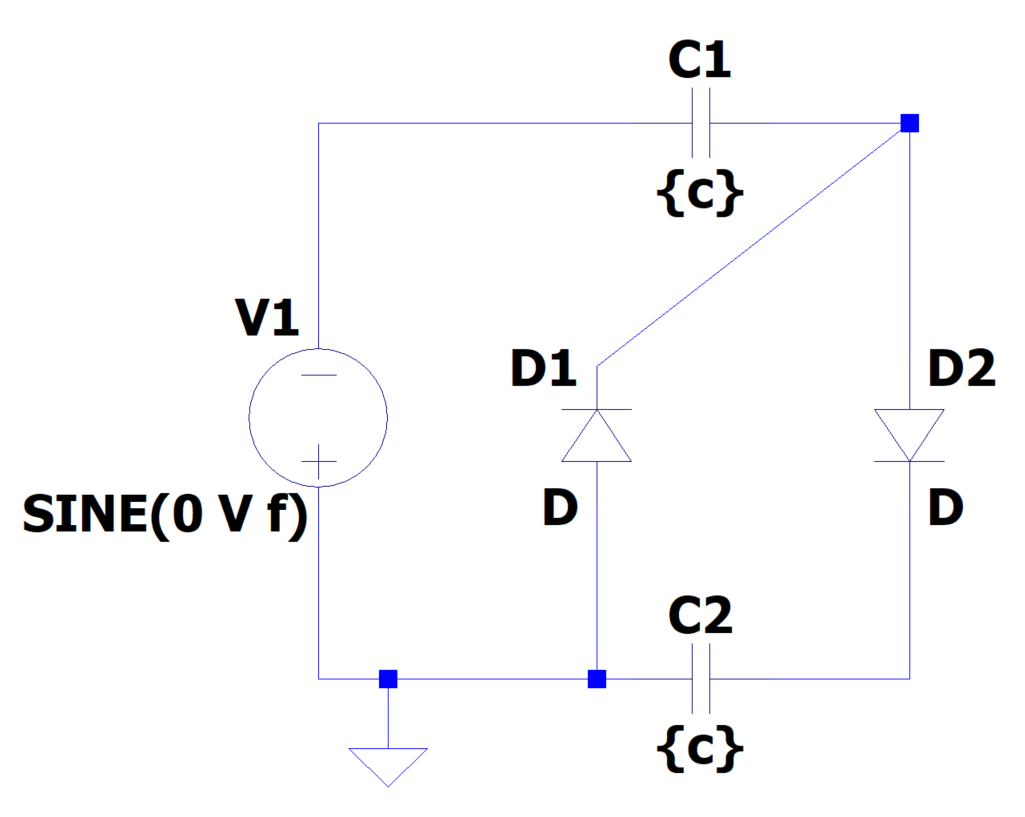
\includegraphics[width=0.6\textwidth]{Imagenes_alvaro/fig_intro.png}
    \caption{Multiplicador de Greinacher de 1 etapa}
    \label{fig_intro}
\end{figure}

Además, cabe destacar que este circuito es escalable, permitiendo de manera teórica obtener tensiones de salida infinitas a partir de fuentes de tensión
oscilatorias de bajo voltaje.

\section{Objetivos}

El principal objetivo de este trabajo es conseguir diseñar un Multiplicador de Greinacher que permita obtener una tensión de salida específica.
Además, debe ser capaz de proveer cierta cantidad de corriente de salida sin que se produzca una caída significativa de la tensión, de manera que será
necesario dimensionar correctamente la capacidad de los condensadores. Por otra parte, el circuito debe ser capaz de funcionar en un rango de frecuencia definido
y para tensiones de entrada senoidales y cuadradas. También será necesario diseñar un circuito que permita medir la tensión de salida a partir de un multímetro.
Todos los requisitos se definen de manera específica en la sección \ref{requisitos}.

\section{Estado de la técnica}

Para la construcción del Multiplicador de Greinacher será necesario obtener el número de etapas necesarias a partir de la tensión de pico de entrada y
la tensión continua requerida a la salida. A partir de ahí se seleccionarán los componentes (diodos y condensadores), los cuales deben ser capaces de soportar las tensiones máximas
a las que se puedan someter.

Respecto a la carga, puesto que la tensión de salida es continua, se dimensionará una resistencia para que circule a través de la misma la corriente deseada.
Dicha resistencia, en el circuito real, deberá ser seleccionada para que pueda soportar la potencia a disipar. Puesto que la tensión de salida será elevada,
corrientes de miliamperios pueden producir potencias de decenas de vatios que deberán ser disipadas por la resistencia.

Para el diseño del circuito de medida de tensión, se utilizará un divisor resistivo con un multímetro en paralelo con la resistencia de debajo del divisor.
De esta manera, la resistencia total de debajo del divisor estará limitada por la resistencia del multímetro. Consecuentemente, puesto
que se debe construir el circuito para obtener corrientes mínimas, se diseñará para que la resistencia de debajo del puente total sea lo más cercana posible a la
resistencia del multímetro.

\section{Establecimiento de requerimientos} \label{requisitos}

Los requerimientos del circuito se dividen, en este caso, en los requerimientos del Multiplicador de Greinacher y los del equipo de monitorización
de tensión de salida. Los requerimientos del Multiplicador de Greinacher son los siguientes:

\begin{itemize}
    \item Tensión de salida: $3kV \pm 5\%\,\, \left(DC\right)$
    \item Corriente de salida: $~5mA$
    \item Rizado máximo: $\pm 10\%$
    \item Tensión de entrada: $220V\,\, \left(AC\right)$
    \item Tensión de trabajo de componentes: $<1000V$
    \item Rango de frecuencia de entrada: $\left[50Hz, 200Hz\right]$
    \item Forma de tensión: senoidal o cuadrada
\end{itemize}

Respecto al equipo de monitorización, debe cumplir los siguientes requisitos para que el funcionamiento del circuito se vea 
lo menos afectado posible al utilizarlo:

\begin{itemize}
    \item Consumo de corriente mínimo
    \item Tensión máxima de $200V$, correspondiente con la tensión máxima de salida
\end{itemize}